%!TEX root = ../TTT4150-Summary.tex
\section{Loxodromes}

A \emph{loxodrome} curve is an Earth course of constant bearing (also called a rhumb). Generally not a great circle, and therefore not the shortest route, but easy to use, as great circles require continuous change of bearing.

%%%%%%%%%%%%%%%%%%%%%%%%%%%%%%%%%%%%%%%%%%%%%%%%%%%%%%%%%%%%
\subsection{Conformal maps}

A \emph{conformal map} distorts east-west and north-south by the same amount, which means that it preserves angles. Distortion depends only on position (actually only latitude). The \emph{Mercator map} is a special conformal map, on which a rhumb/loxodrome is a straight line.

\begin{figure}[htbp]
	\centering
	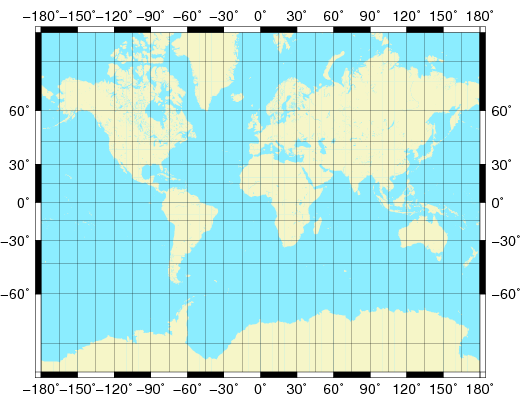
\includegraphics[width=\linewidth]{img/esa_mercator_map}
	\caption{A Mercator map}
\end{figure}
